\section{Extraktion des Nummernschildes}

\begin{frame}{Convolutional Neural Networks}
    \begin{figure}
        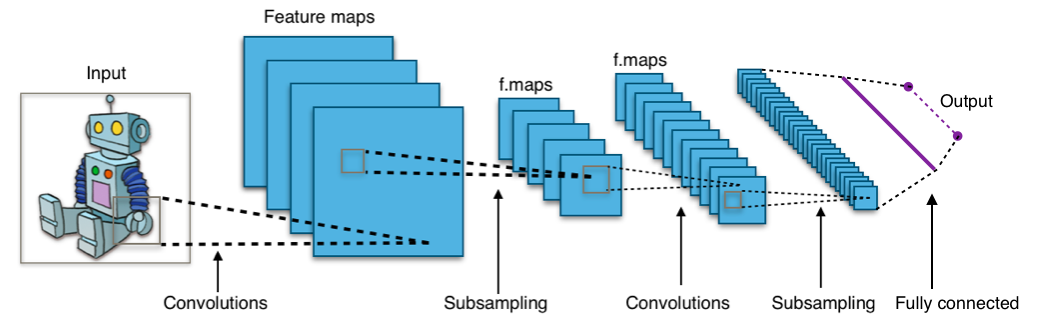
\includegraphics[width=\textwidth]{bilder/Typical_cnn.png}
        \caption{Convolutional Neural Network.
            \footnote{Bildquelle: \url{https://de.wikipedia.org/wiki/Convolutional_Neural_Network}}}
    \end{figure}
    \begin{center}
        \fbox{\textbf{Input:} Bild mit Auto $\longmapsto$ \textbf{Output:} Bounding Box}
    \end{center}
\end{frame}

\begin{frame}{Implementierung}
    \textbf{Netzarchitektur:}
    \begin{itemize}
        \item Inspiriert durch YOLO (\textbf{Y}ou \textbf{O}nly \textbf{L}ook \textbf{O}nce) \cite{yolov3}
        \item Kann sowohl Klassen als auch Bounding Boxes vorhersagen
        \begin{itemize}
            \item[$\rightarrow$] Wir brauchen nur Bounding Boxes von Nummernschildern, also Vereinfachung n\"otig
        \end{itemize}
    \end{itemize}
    \textbf{Implementierung:}
    \begin{itemize}
        \item Open Source Deep-Learning Bibliothek Keras
        \item Geschrieben in Python
    \end{itemize}
\end{frame}